\documentclass[10pt,conference,compsocconf]{IEEEtran}

\usepackage{hyperref}
\usepackage{graphicx}	% For figure environment
\usepackage{natbib}
\usepackage{float}
\usepackage{hyperref}
\usepackage{url}

\begin{document}
\title{Process Book}

\author{
  Rehan Mulakhel, Noemi Romano, Raja Soufi\\
  \textit{Department of Computer Science, EPFL Lausanne, Switzerland}
}

\maketitle

\begin{abstract}
A critical part of scientific discovery is the communication of research findings to peers or the general public. Mastery of the process of scientific communication improves the visibility and impact of research. While this guide is a necessary tool for learning how to write in a manner suitable for publication at a scientific venue, it is by no means sufficient, on its own, to make its reader an accomplished writer. This guide should be a starting point for further development of writing skills.
\end{abstract}

\section{Introduction}

Over human history, thousands and thousands of meteorites fell to the Earth ground; chunk of rock and metal disagreggating in the atmosphere, hitting the ground and causing sometimes vast disasters. 

The goal of this project is to visualize this fascinating phenomenon occurred over the last centuries by means of georeferenced location of the impacts recorded by the \textit{Meteoritical society}\footnote{Meteoritical society: \href{http://www.meteoriticalsociety.org/}{http://www.meteoriticalsociety.org/}}. In this visualization, our principal aim is to give a general overview of the spatio-temporal evolution of this natural phenomenon, emphasizing on the user experience and the exploration of the data. This visualization targets a general public who has not strong knowledge in the field. 


\section{Data}
\label{sec:data}
The data come from the NASA’s Open Data Portal and have been downloaded from Kaggle’s platform. The data were collected by The Meteoritical Society and contain information on all of the known meteorite landings. The dataset includes the following fields:

\begin{description}
\item[\texttt{name}] \ \\
  The name of the meteorite (typically a location, often modified with a number, year, composition, etc).
\item[\texttt{id}] \ \\
  The unique identifier for the meteorite.
\item[\texttt{nametype}] \ \\
  One of: -- \texttt{valid}: a typical meteorite -- \texttt{relict}: a meteorite that has been highly degraded by weather on Earth.
\item[\texttt{recclass}] \ \\
  The class of the meteorite; one of a large number of classes based on physical, chemical, and other characteristics.
\item[\texttt{mass}] \ \\
  The mass of the meteorite, in grams.
\item[\texttt{fall}] \ \\
   Whether the meteorite was seen falling, or was discovered after its impact; one of: -- Fell: the meteorite's fall was observed -- Found: the meteorite's fall was not observed.
\item[\texttt{year}] \ \\
  The year the meteorite fell, or the year it was found (depending on the value of fell).
\item[\texttt{reclat}] \ \\
  The latitude of the meteorite's landing.
\item[\texttt{reclong}] \ \\
  The longitude of the meteorite's landing.
\item[\texttt{GeoLocation}] \ \\
  The parentheses-enclose, comma-separated tuple that combines \texttt{reclat} and \texttt{reclong}.
\end{description}

Rows containing \texttt{NaN} values or presenting a year’s value smaller than $1800$ and bigger than $2013$ will not be considered in our visualization project. In addition, some of the entries having coordinates values equal to $0$ ---referring to meteorites found in Antarctica of which coordinates were not given--- will not be considered. 

% TODO: topojson & three

After the cleaning, we end up with a final number of $31,705$ over $45,716$ entries.

\section{Tools}
\label{sec:tools}

The visualization is displayed in a browser for usability reasons: users do not need to download anything. This forces the application to be split into a front-end and a back-end.

\subsection{Front-end}

The main visualization of the globe and falling meteorites is done with \href{https://threejs.org/}{Three.js}.
The rest of the visualizations (timeline, class statistics, etc.) were done with \href{https://d3js.org/}{D3} and \href{http://vizjs.org/}{viz.js}.

jQuery and Bootstrap were also used.

\subsection{Back-end}

Most files necessary for displaying the web page are served using GitHub pages (the libraries being fetched from various CDNs except for viz.js).

All the data related to meteorites and countries is saved on Google Drive and served using a simple Google Apps Script web app, which also provides a few endpoints to get filtered or grouped data (see \href{https://github.com/RajaSoufi/GeoMeteorites/tree/master/gds-doc#google-drive-server-documentation}{here}).

\newpage
\section{Evolution of visualization}
\label{sec:evolution_of_visualization}

The first step was to figure out which visualization could be appropriate to visualize the spatial distribution of the meteorites' impacts. A globe or a map with the georeferenced impacts as static points came to our mind, but the UX would have been limited. That's why we decided to animate the trajectory of the meteorite falls, in order to give a realistic dimension to the data. In order to enforce the realistic dimension we prioritized the 3D visualization, hence a globe has been chosen to visualize the geographical space. To give a more global point of view of the spatial distribution of this phenomena, the transition from the globe to a 2D map has been also taken into account. 

Having the coordinates of the impacts, it was crucial to get the country where the meteorites fell. Getting access to the country implies then a new category of classification, leading to a local and easier exploration of the data. The local dimension gave us new ideas for the data representation: 

\begin{itemize}
\item Visualization of the country related statistics
\item A search-bar where the user can enter the country wished
\item The interaction user-globe that allows to click over a country and see the meteorites falling for the country selected 
\item Histogram of the type of meteorite by country
\end{itemize}

A time-line was by far the easiest way to visualize the temporal dimension. In order to add an interaction to it, we decided to allow the selection of an interval of time to the user. The animation of the meteorites falls will be then performed in the interval of time selected and activated/deactivated with a start/pause button. 

Here below our first sketch of the visualization:
\iffalse
\begin{figure}[H]
  \centering
  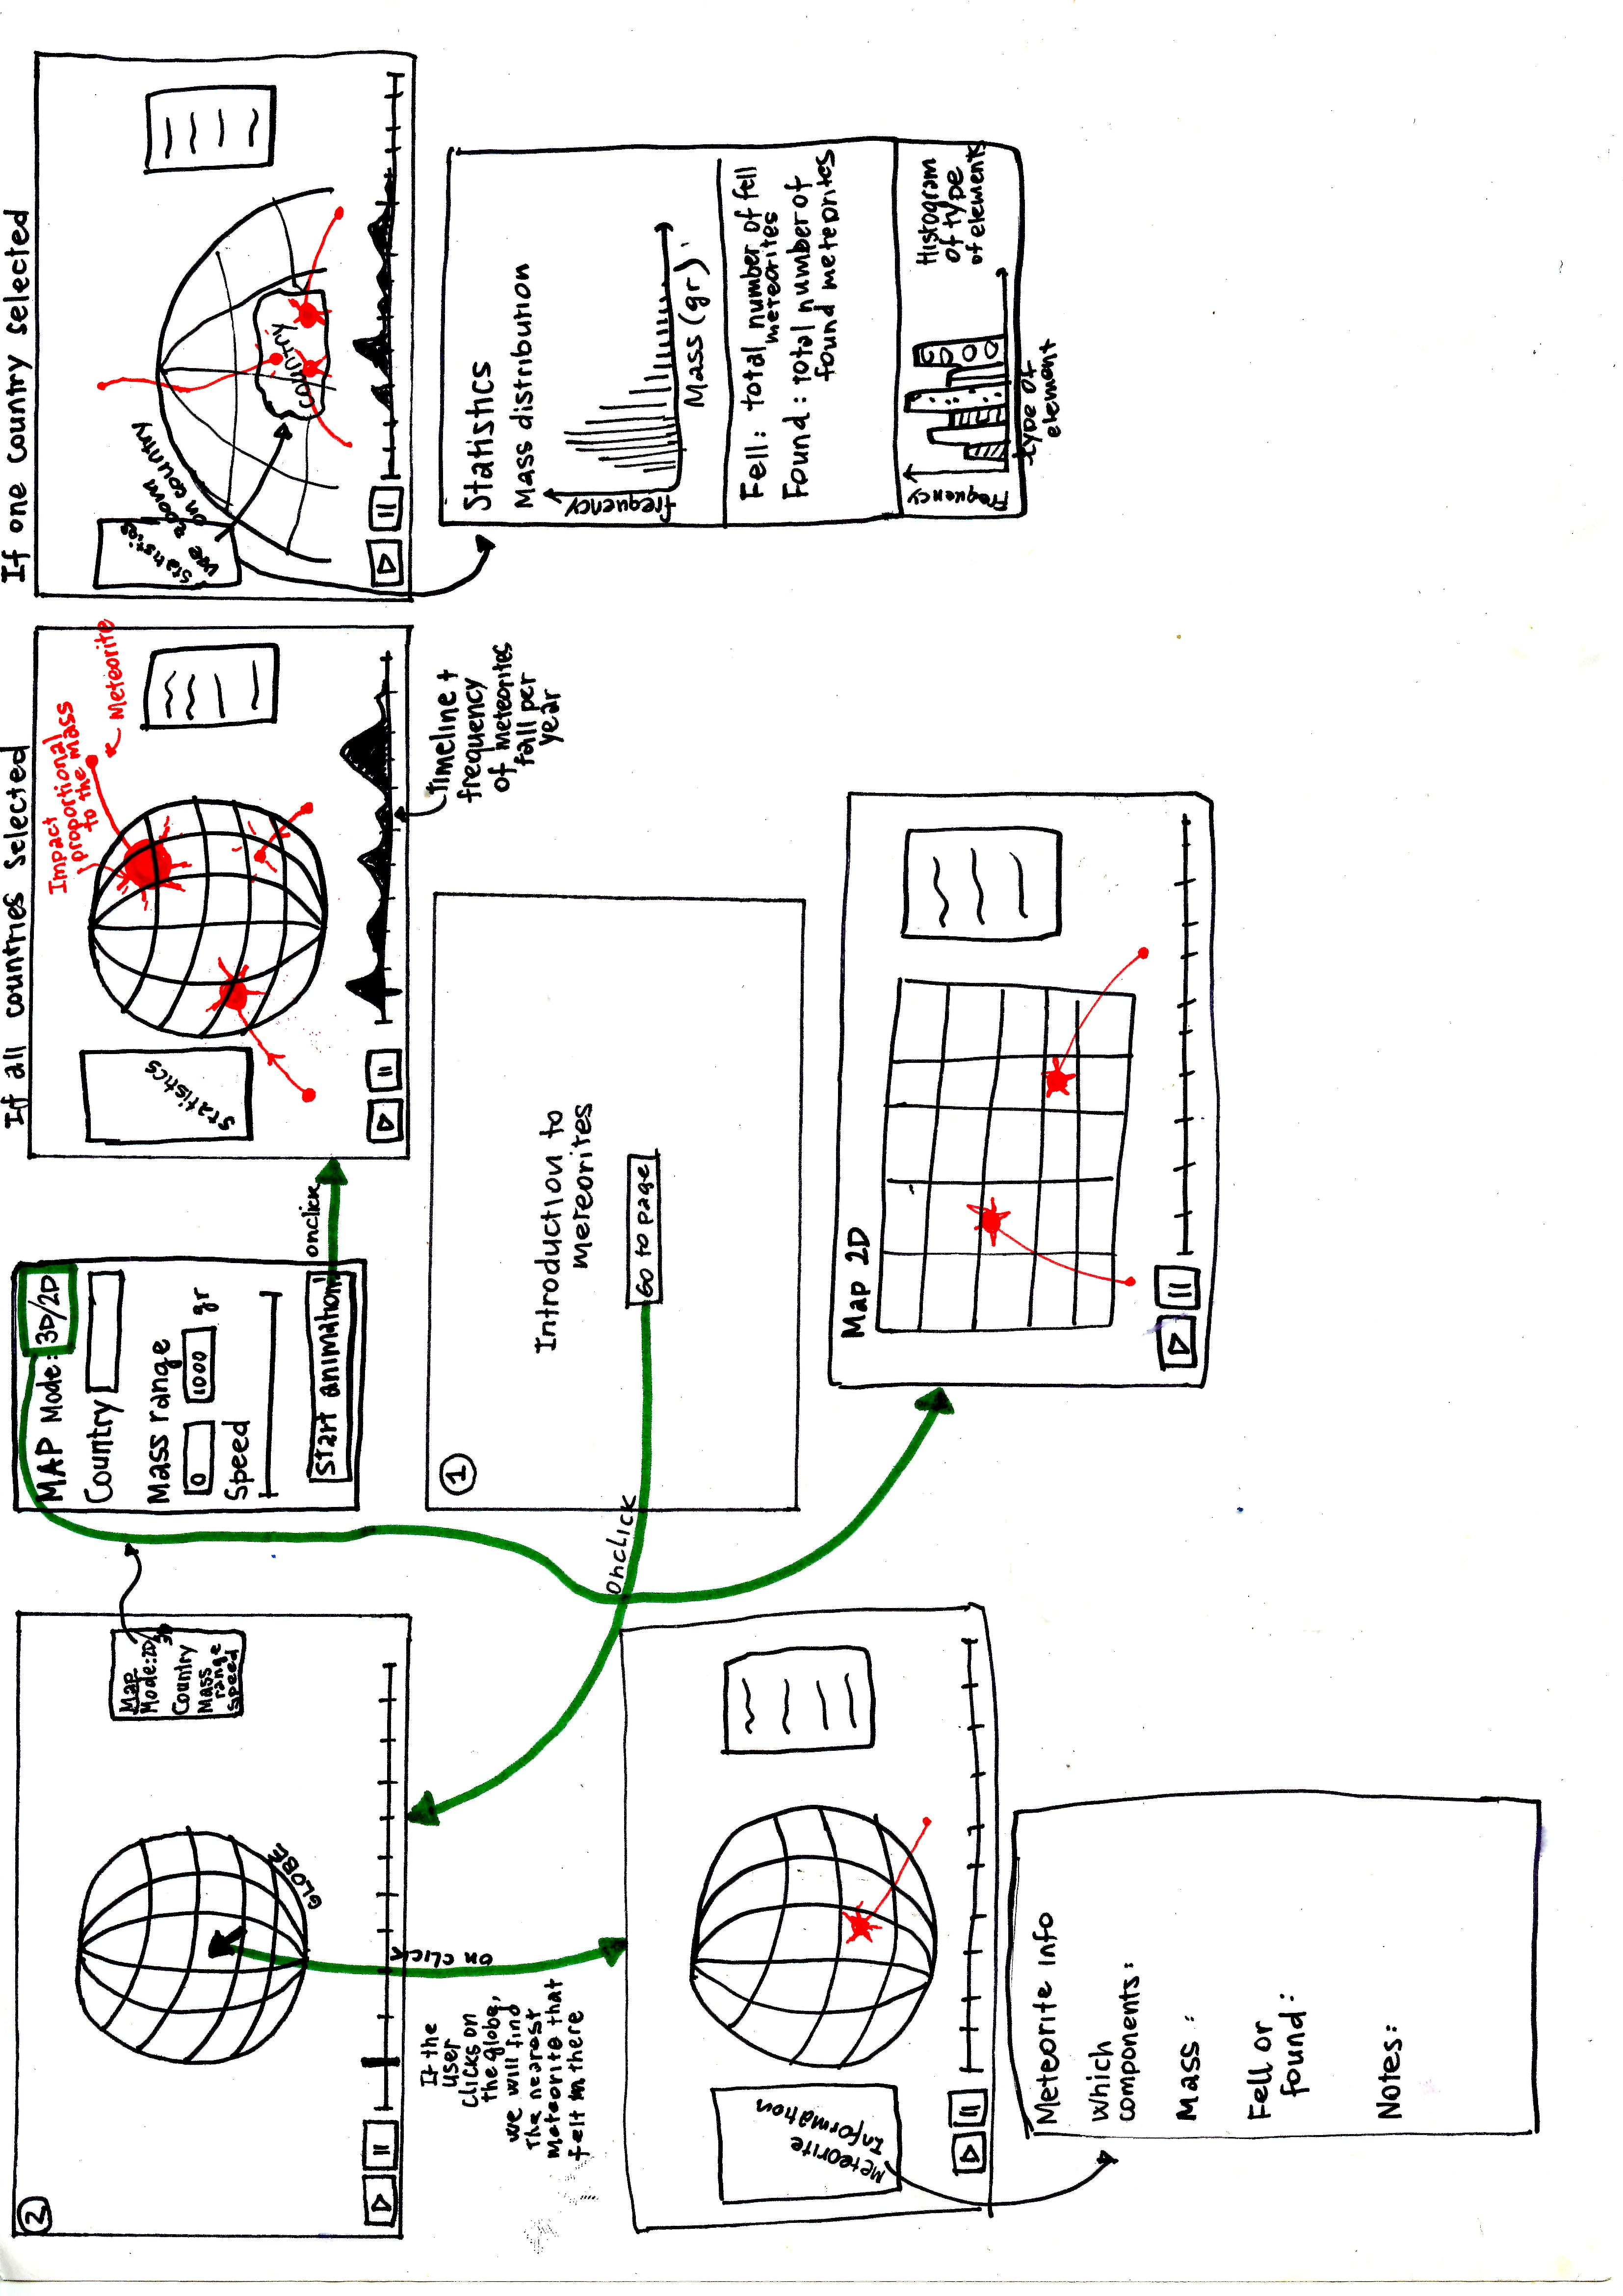
\includegraphics[width=\columnwidth]{sketch1}
  \vspace{-3mm}
  \caption{First sketch of the visualization}
  \label{fig:denoise-wavelet}
\end{figure}
\fi


\subsection{Globe}
Exploring the Mike Bostock's Blocks \cite{bostock_mike_nodate} we discovered many tutorial allowing the creation of a globe with $d3.js$ \cite{bostock_see-through_nodate,bostock_globe_nodate}.  These works are performed with the \texttt{d3.geo} library that allows an easy way to work with geographic information and different projections.

We then created the globe, but a sticking point came up: how to handle the meteorites' animation with \texttt{d3}?

We then explored other javascript libraries that could handle in a simpler way the animation of 3D objects and we figured out that the \texttt{three.js} library \cite{BibEntry2017Nov} is the most suitable one (explain why).

We inspired our globe from another Mike Bostock example \cite{BibEntry2017Aug} that shows how to import \texttt{geoJSON} files in a \texttt{three.js} scene. The \texttt{three} library doesn't read automatically objects with geometry as \texttt{d3} does. First of all, the \texttt{geoJSON} file containing the countries borders' multilinestring \cite{countryfile} and re-projected the coordinates of the latter into spherical projection. Then, all the starting and ending vertices of the multilinestring have to be pushed in a \texttt{three geometry} and a line has to be drawn between all these couples of vertices.

%Speak about the graticule TODO
he graticule was drawn...\\

A white sphere has been added as well in order to do not see through the globe.
We finally ended up with the following globe:
\begin{figure}[H]
  \centering
  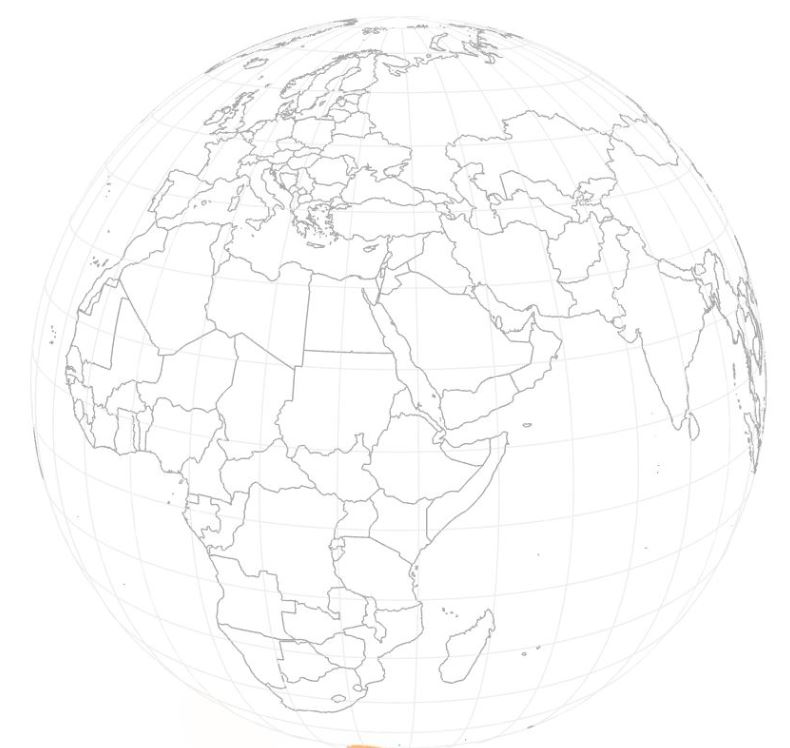
\includegraphics[width=\columnwidth]{globe.jpg}
  \vspace{-3mm}
  \caption{Globe with $three.js$}
  \label{fig:globe}
\end{figure}

In order to add an interaction to the globe, the user can zoom-in, zoom-out, and drag the globe. 
The 2D map has also been taken into account, but being our first aim to make this visualization as realistic as possible, we finally decided to keep only the globe.

\subsection{Meteorites' country}

The original data set provided by Kaggle did not contain any information on countries name. The only way to map a country to a landing was through the geo coordinates. Since the \texttt{csv} file contains many thousands rows, it was impossible to do it manually. This lead us to write a script in python in order to fetch countries based on the tuple (latitude, longitude).

Google Maps, which is likely to be the most famous web app for location, has its services limited to users to avoid DDoS\footnote{Distributed Denial of Service} attack. According to their documentation, the number is limited to a ``a few thousands'' requests by day per person. This could have taken more than one week to get our new data! Clearly, we had to find a solution. That's why we dropped the idea of Google Maps and turned towards Open Street Map, an open source alternative.

Open Street Map also has a system to prevent DDoS attack. But it does not have a limited number of requests per day. Actually their api sends the error $429$ which stands for ``too many requests'', requiring the script to block for several minutes. Eventually the script was run on a server for more than thirty hours.

%Second process

\subsection{Time-line}

The first idea was to create an animation close to a video. The starting and the ending moments were supposed to be parameters. The inspiration came from \cite{ocks_brush_and_zoom}, parts of the code were taken and adapted to the latest version of ES6\footnote{ECMAScript 6}. There was a plot of the number of meteorites group by year inside the time-line. 

The data contains date from 860 to 2016. The plot shows that most meteorites hit the Earth recently. This is unlikely to be the reality. We can interpret it like humans have almost no information on the subject until the 19\textsuperscript{th} century. This information leads us to filter from ?? to 2016.

When the application started to work with the globe and the meteorites hitting it. It became obvious selecting the time range was not user friendly. Instead, a flag with the `current' year (of the animation) is moving like a cursor which can be dragged and dropped. This way, only one button to start and stop is needed.

\subsection{Meteorites animation}


\subsection{Search bar}


\subsection{Meteorites classification}


\subsection{Country statistics}


\subsection{Story telling}
Speak about the messages. 

\subsection{Final touches}
Night-day texture
Layout






\section{Improvements}
\label{sec:improvements}

To do.

\section{Work split}
\label{sec:work_split}

\begin{description}
\item[Rehan Mulakhel] \ \\
  Web page centralizing links to the demo, code and process book. General design of the demo page. Brushing time line. Dynamic suggestion for the countries. Country to each meteorite based on coordinates. 
\item[Noemi Romano] \ \\
  To do.
\item[Raja Soufi] \ \\
  Globe visualization (partly) as well as falling meteorites and world camera animations/movements.
  Improvements to various elements such as timeline and search field, as well as linking the various parts together.
\end{description}




\bibliography{geometeorites}
\bibliographystyle{plain}



\end{document}
